%%%%%%%%%%%%%%%%%%%%%%%%%%%%%%%%%%%%%%%%%%%%%%%%%%%
%% P3: Phenomenology of Particle Physics                         
%%
%% Author:  André Rubbia                   		 
%%
%% Figure 28.11 Graphical representation of the kinematical plane $Q^{2}$ vs. $2 M \nu$.
%%
%% This work is licensed under the Creative Commons Attribution 4.0 International License. 
%% To view a copy of this license, visit http://creativecommons.org/licenses/by/4.0/ or 
%% send a letter to Creative Commons, PO Box 1866, Mountain View, CA 94042, USA.
%%
%%%%%%%%%%%%%%%%%%%%%%%%%%%%%%%%%%%%%%%%%%%%%%%%%%%

\documentclass[a4paper,10pt]{article}

\usepackage[T1]{fontenc}
\usepackage[utf8]{inputenc}
\usepackage{lmodern}
\usepackage[labelfont=bf]{caption}
\usepackage{upgreek}

\usepackage{amssymb}
\usepackage{amsmath}
\usepackage{mathtools}

\usepackage{tikz}
\usepackage{pgfplots}
\pgfplotsset{compat=1.17}
\usepgfplotslibrary{ternary}
\usepgfplotslibrary{fillbetween}
\usepgfplotslibrary{external}

\def\d{\mathrm{d}}
\setlength{\oddsidemargin}{-1.0cm}
\setlength{\evensidemargin}{-1.0cm}
\setlength{\textheight}{25cm}
\setlength{\textwidth}{18cm}

\pgfkeys{/pgf/number format/.cd,1000 sep={}}

\begin{document}

%%%%%%%%%%%%%%%%   FIGURE  %%%%%%%%%%%%%%%%%%%%%%%%%%%%%%
\begin{figure}[htb]
	\centering
\begin{tikzpicture}[scale=1.]
\begin{axis}[xbar,
	height=8cm, width=8cm,
    	symbolic x coords={0,$2ME_\nu$},
  	xtick={0,$2ME_\nu$},
	xmin=0,xmax=$2ME_\nu$,
    	symbolic y coords={0,$2ME_\nu$},
  	ytick={0,$2ME_\nu$},
	ymin=0,ymax=$2ME_\nu$,
%	title=Pion decay,
	xlabel=$2M\nu$,
	ylabel=$Q^2$,
	legend pos = north west] {};
	 \draw[black, very thick] (axis cs:0,0) -- (axis cs:$2ME_\nu$,$2ME_\nu$);
\end{axis}
	 \draw[black, very thick] (3.3,3.75) node[rotate=45] {$W^2=M^2$, $x=1$};
	 \draw[black, very thick] (3.3,2.8) node[rotate=45] {Threshold for single pion};
	 \draw[magenta,  thick] (4.5,2) node[rotate=45] {$W^2=\text{constant}$};
	 \draw[black,  thick,dashed] (1,0) -- +(5.4,5.4);
	 \draw[magenta,  thick] (3,0) -- +(3.4,3.4);
	 \draw[blue,  thick] (6,0) -- +(0,6);
	 \draw[red,  thick] (0,0) -- +(6.4,1);
	 \draw[red,  thick] (4.95,0.62) node[rotate=9] {$x=\text{constant}$};
	 \draw[blue,  thick] (6.2,2) node[rotate=90] {$y=\text{constant}$};
\end{tikzpicture}
	\caption{Graphical representation of the kinematical plane $Q^{2}$ vs. $2 M \nu$.}
\end{figure}
%
%%%%%%%%%%%%%%%%   END FIGURE  %%%%%%%%%%%%%%%%%%%%%%%%%%%%%%
%


\end{document}
